\scanpage{18}
cette dernière, si $\operatorname{card}J=\operatorname{card}I-1=n-1$, on verra (par r\unsure{è|é}currence) que le cardinal de l'ens des classes est $(n-1)+1=n$.

Ceci posé, on voit d'abord que $E_i$ est dans
% G01: original full-scan origin (820,455); x=0.010cm, y=-0.010cm.
% Fixed drawing rectangle 670 by 160 source-coordinate units. The words occur here once.
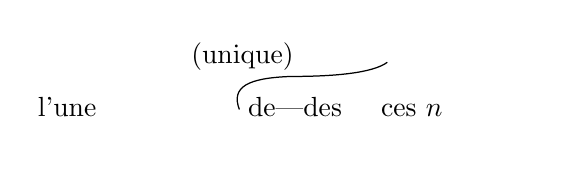
\begin{tikzpicture}[x=.010cm,y=-.010cm,baseline=(g01base)]
\path[use as bounding box] (0,0) rectangle (670,160);
\coordinate (g01base) at (0,113);
\begin{scope}[shift={(-820,-455)}]
\node[anchor=base west,inner sep=0pt,outer sep=0pt] at (833,568) {l'une};
\node[anchor=base west,inner sep=0pt,outer sep=0pt] at (1100,568) {\unsure{de|des}};
\node[anchor=base west,inner sep=0pt,outer sep=0pt] at (1269,568) {ces $n$};
\node[anchor=base west,inner sep=0pt,outer sep=0pt] at (1028,500) {\inserted{(unique)}};
% G01a: complete long insertion guide, with bent left end and upturned right end.
\draw[line width=.45pt] (1089,559) .. controls (1078,530) and (1100,519) .. (1154,517) .. controls (1208,517) and (1258,513) .. (1277,499);
\end{scope}
\end{tikzpicture}
classes, qui sont des ouverts. Soit $U_{J,i}$ la classe (ou ``composante'') qui contient $E_i$, et considérons les deux composantes $\Sigma_i^+,\Sigma_i^-$ de $X\setminus E_i$.

% G02: complete two-line lemma group; full-scan origin (230,1135).
% x=0.010cm, y=-0.010cm; fixed 1410 by 270 source-coordinate rectangle.
\figure{\begin{tikzpicture}[x=.010cm,y=-.010cm]
\path[use as bounding box] (0,0) rectangle (1410,270);
\begin{scope}[shift={(-230,-1135)}]
\node[anchor=base west,inner sep=0pt,outer sep=0pt] at (300,1250) {\rlap{Lemme}\phantom{\uline{Lemme}}};
\node[anchor=base west,inner sep=0pt,outer sep=0pt] at (640,1238) {Toute classe de $\Pi_{J\deleted{\unsure{i|j|,}}}^{\unsure{\circ|0}}$, distincte};
\node[anchor=base west,inner sep=0pt,outer sep=0pt] at (275,1376) {de $U_{J,i}$, est contenue dans $\Sigma_i^+$ ou $\Sigma_i^-$};
% G02a: heading underline; G02b: separate, short left rule.
\draw[line width=.5pt] (307,1275) .. controls (382,1268) and (467,1262) .. (550,1258);
\draw[line width=.5pt] (254,1248) .. controls (255,1299) and (257,1351) .. (259,1383);
\end{scope}
\end{tikzpicture}}

C'est presque une tautologie : Dire
% G03: qu'une/la/classe group, full-scan origin (235,1480), fixed 310 by 125 rectangle.
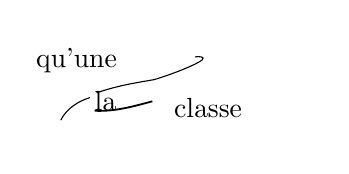
\begin{tikzpicture}[x=.012cm,y=-.012cm,baseline=(g03base)]
\path[use as bounding box] (0,0) rectangle (310,125);
\coordinate (g03base) at (0,91);
\begin{scope}[shift={(-235,-1480)}]
\node[anchor=base west,inner sep=0pt,outer sep=0pt] at (244,1522) {\inserted{qu'une}};
\node[anchor=base west,inner sep=0pt,outer sep=0pt] at (306,1568) {\rlap{la}\phantom{\deleted{la}}};
\node[anchor=base west,inner sep=0pt,outer sep=0pt] at (390,1575) {classe};
% G03a/b: observed interrupted insertion guide; the q descender belongs to qu'une.
\draw[line width=.4pt] (270,1578) .. controls (276,1566) and (288,1558) .. (301,1554);
\draw[line width=.4pt] (308,1549) .. controls (331,1541) and (352,1538) .. (369,1535) .. controls (389,1529) and (414,1519) .. (420,1514) .. controls (423,1511) and (417,1510) .. (412,1511);
% G03c: the actual lower cancellation stroke, without an additional generic rule.
\draw[line width=.65pt] (306,1568) .. controls (328,1569) and (348,1563) .. (367,1558);
\end{scope}
\end{tikzpicture}
% G04: donnée / inserted name / ne group. Full-scan origin (530,1445), fixed 525 by 160.
\begin{tikzpicture}[x=.010cm,y=-.010cm,baseline=(g04base)]
\path[use as bounding box] (0,0) rectangle (525,160);
\coordinate (g04base) at (0,111);
\begin{scope}[shift={(-530,-1445)}]
\node[anchor=base west,inner sep=0pt,outer sep=0pt] at (560,1556) {donnée};
\node[anchor=base west,inner sep=0pt,outer sep=0pt] at (797,1548) {ne};
\node[anchor=base west,inner sep=0pt,outer sep=0pt] at (737,1507) {\inserted{$U_{\unsure{\alpha|x}}$\quad de $\Pi_J^\circ$}};
% G04a: complete guide; no separate cancelled un is supplied.
\draw[line width=.4pt] (761,1554) .. controls (762,1540) and (791,1528) .. (811,1516) .. controls (853,1528) and (876,1534) .. (908,1521) .. controls (957,1511) and (1006,1500) .. (1012,1487);
% G04b: one locally qualified comma-like hook at the guide junction.
% Nested local origin (806,1504), baseline (0,0), base-west placement and zero separation.
% Its role as comma or guide return is unsettled; no second printed comma is added.
\node[anchor=base west,inner sep=0pt,outer sep=0pt] at (806,1504) {\unsure{\begin{tikzpicture}[x=.010cm,y=-.010cm,baseline=(g04hookbase)]
\path[use as bounding box] (0,0) rectangle (15,17);
\coordinate (g04hookbase) at (0,0);
\draw[line width=.45pt] (0,4) .. controls (9,0) and (15,6) .. (6,13);
\end{tikzpicture}}};
\end{scope}
\end{tikzpicture}
contient pas $\deleted{\Sigma}\overline{E_i}$ i.e. est $\ne U_{J,i}$, signifie que il existe un $j\in J$ tel que le $\Sigma_j^+\in\pi_0(X\setminus\deleted{\Sigma}E_j)$
% G05: cancelled word and two detached endpoint points, origin (1400,1715), fixed 200 by 90.
\begin{tikzpicture}[x=.012cm,y=-.012cm,baseline=(g05base)]
\path[use as bounding box] (0,0) rectangle (200,90);
\coordinate (g05base) at (0,49);
\begin{scope}[shift={(-1400,-1715)}]
\node[anchor=base west,inner sep=0pt,outer sep=0pt] at (1410,1764) {\rlap{\unsure{choisi|choisie}}\phantom{\deleted{\unsure{choisi|choisie}}}};
% G05a: single cancellation stroke.
\draw[line width=.6pt] (1410,1757) .. controls (1468,1756) and (1524,1757) .. (1566,1758);
% G05b/c: both extra endpoint points occur once; the two i dots stay within the word.
% Nested origin (1567,1745), baseline (0,0), base-west anchor and zero separation.
\node[anchor=base west,inner sep=0pt,outer sep=0pt] at (1567,1745) {\unsure{\begin{tikzpicture}[x=.012cm,y=-.012cm,baseline=(g05pointsbase)]
\path[use as bounding box] (0,0) rectangle (12,12);
\coordinate (g05pointsbase) at (0,0);
\fill (2,8) circle[radius=1.1];
\fill (9,2) circle[radius=1.0];
\end{tikzpicture}}};
\end{scope}
\end{tikzpicture}
``composant'' de cette classe \deleted{est} est l'\unsure{é|e}l\unsure{é|ê}ment du $\pi_0$ qui ne contient pas $E_i$; il est donc contenu dans l'un des
% G06: whole éléments / (soit Sigma) / de / pi_0 group, origin (245,2135), fixed 795 by 155.
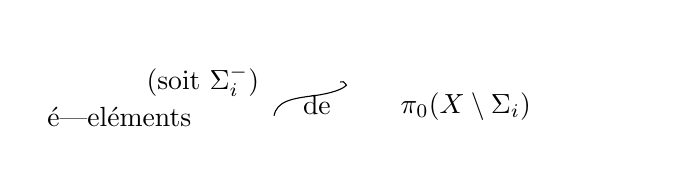
\begin{tikzpicture}[x=.010cm,y=-.010cm,baseline=(g06base)]
\path[use as bounding box] (0,0) rectangle (795,155);
\coordinate (g06base) at (0,125);
\begin{scope}[shift={(-245,-2135)}]
\node[anchor=base west,inner sep=0pt,outer sep=0pt] at (270,2260) {\unsure{é|e}léments};
\node[anchor=base west,inner sep=0pt,outer sep=0pt] at (396,2213) {\inserted{(soit $\Sigma_i^-$)}};
\node[anchor=base west,inner sep=0pt,outer sep=0pt] at (595,2245) {de};
\node[anchor=base west,inner sep=0pt,outer sep=0pt] at (719,2244) {$\pi_0(X\setminus\Sigma_i)$};
% G06a: guide crossing the ascender of de, with its full right hook.
\draw[line width=.4pt] (558,2247) .. controls (562,2228) and (580,2225) .. (612,2221) .. controls (632,2218) and (646,2213) .. (650,2208) .. controls (647,2204) and (645,2202) .. (642,2204);
\end{scope}
\end{tikzpicture}, d'après l'étude du
% G07: cas / cancelled deux / raised card I=2, origin (245,2240), fixed 370 by 123.
\begin{tikzpicture}[x=.012cm,y=-.012cm,baseline=(g07base)]
\path[use as bounding box] (0,0) rectangle (370,123);
\coordinate (g07base) at (0,85);
\begin{scope}[shift={(-245,-2240)}]
\node[anchor=base west,inner sep=0pt,outer sep=0pt] at (275,2325) {cas};
\node[anchor=base west,inner sep=0pt,outer sep=0pt] at (400,2321) {\rlap{\unsure{deux}}\phantom{\deleted{\unsure{deux}}}};
\node[anchor=base west,inner sep=0pt,outer sep=0pt] at (386,2302) {\inserted{$\operatorname{card}I=2$}};
% G07a: complete long cancellation rule, kept once.
\draw[line width=.65pt] (399,2320) .. controls (438,2313) and (483,2317) .. (515,2314) .. controls (531,2312) and (546,2311) .. (555,2312);
% G07b: supported lower hook below the I/= region; its guide/letter role remains unsettled.
% Nested origin (510,2290), baseline (0,0), base-west placement and zero separation.
\node[anchor=base west,inner sep=0pt,outer sep=0pt] at (510,2290) {\unsure{\begin{tikzpicture}[x=.012cm,y=-.012cm,baseline=(g07hookbase)]
\path[use as bounding box] (0,0) rectangle (12,27);
\coordinate (g07hookbase) at (0,0);
\draw[line width=.5pt] (4,4) .. controls (10,10) and (8,18) .. (1,24);
\end{tikzpicture}}};
\end{scope}
\end{tikzpicture}, \deleted{\unsure{OK|cela}} \unsure{â|à} fortiori $U_\alpha\subset\Sigma_i^-$, OK.
% archive sheet number: 17
